\documentclass[11pt]{article}

\author{wilricknl}
\title{3D Math Primer - Solutions chapter 7}

\usepackage{amsmath}
\usepackage{amssymb}
\usepackage{float}
\usepackage{enumerate}
\usepackage{graphicx}

\begin{document}

\maketitle

\section{Solutions chapter 7}


\subsection{Exercise 1}

\begin{figure}[H]
\centering
    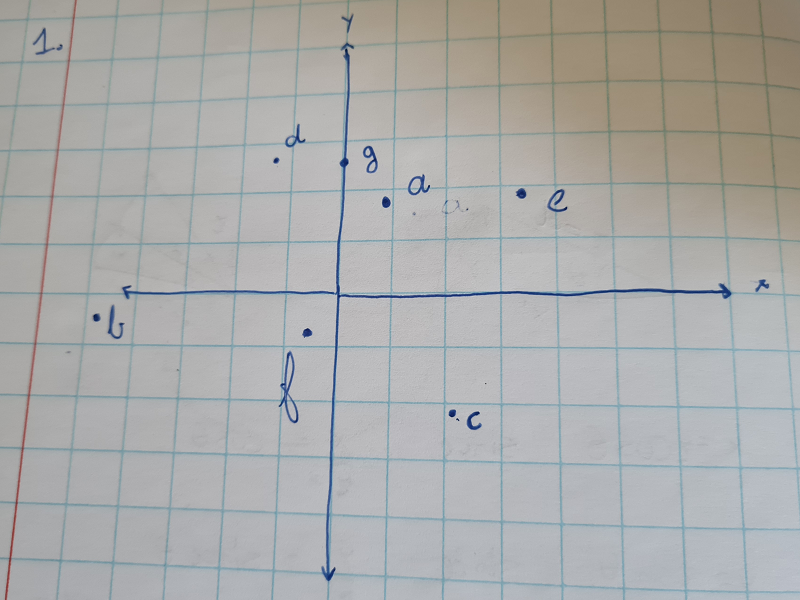
\includegraphics{exercise01}
\caption{Exercise 1}
\label{fig:07-exercise-01}
\end{figure}


\subsection{Exercise 2}

\begin{enumerate}[a.]
	\item % a
	$\theta > 180^\circ$, so $(4, 207^\circ - 360^\circ)= (4,-153^\circ)$.
	\item % b
	$r < 0$, so $((-1)(-5),-720^\circ+180^\circ)=(5, -540^\circ)$\\
	$-540^\circ \leq -180^\circ$, so $(5, -540^\circ+360^\circ)=(5, -180^\circ)$ \\ 
	$-180^\circ \leq -180^\circ$, so $(5, -180^\circ+360^\circ)=(5, 180^\circ)$
	\item % c
	$r = 0$, so $(0,0)$.
	\item % d
	$\frac{11\pi}{4}=2\pi + \frac{3\pi}{4}$, so we can discard one revolution and are left with $(12.6, \frac{3\pi}{4})$.
\end{enumerate}


\subsection{Exercise 3}

\begin{enumerate}[a.]
	\item $((1)\cos\frac{\pi}{4},(1)\sin\frac{\pi}{4})=(\frac{\sqrt{2}}{2},\frac{\sqrt{2}}{2})$
	\item $((3)\cos0,(3)\sin0)=(3,0)$
	\item $(4\cos\frac{\pi}{2},4\sin\frac{\pi}{2})=(0,4)$
	\item $((10)\cos-\frac{\pi}{6},(10)\sin-\frac{\pi}{6})=(5\sqrt{3},-5)$
	\item $(-5.5,0)$
\end{enumerate}


\subsection{Exercise 4}

\begin{enumerate}[a.]
	\item $((4)\cos(207^\circ),(4)\sin(207^\circ))$
	\item $(-5,0)$
	\item $(0,0)$
	\item $((12.6)(-\frac{\sqrt{2}}{2}),(12.6)(\frac{\sqrt{2}}{2}))=(-6.3\sqrt{2},6.3\sqrt{2})$
\end{enumerate}


\subsection{Exercise 5}

\begin{enumerate}[a.]
	\item % a
		\begin{itemize}
			\item $r=\sqrt{10^2+20^2}=\sqrt{500}=10\sqrt{5}$
			\item $\theta=\text{atan2}(20,10)=\arctan(\frac{20}{10}) \approx 63.435^\circ$
		\end{itemize}
	\item % b
		\begin{itemize}
			\item $r=13$
			\item $\theta=\arctan\frac{-5}{-12}-180^\circ \approx -157.38^\circ$
		\end{itemize}
	\item % c
		\begin{itemize}
			\item $r=4.5$
			\item $\theta=90^\circ$, because $x=0$ and $y>0$
		\end{itemize}
	\item % d
		\begin{itemize}
			\item $r=5$
			\item $\theta=\arctan\frac{4}{-3}+180^\circ \approx 126.870$
		\end{itemize}
	\item % e
		\begin{itemize}
			\item $r=0$
			\item $\theta=0$
		\end{itemize}
	\item % f
		\begin{itemize}
			\item $r=5280$
			\item $\theta=180^\circ$, because $x>0$
		\end{itemize}
\end{enumerate}


\subsection{Exercise 6}

\begin{enumerate}[a.]
	\item % a
	$
	\left.
	\begin{aligned}
		x &= (4)\cos 120^\circ = -2 \\
		y &= (4)\sin 120^\circ = 2\sqrt{3} \\
		z &= 5
		\end{aligned}
	\right\}(-2,2\sqrt{3},5)
	$
	\item % b
	$
	\left.
	\begin{aligned}
		x &= (2)\cos 45^\circ = \sqrt{2} \\
		y &= (2)\sin 45^\circ = \sqrt{2} \\
		z &= -1
		\end{aligned}
	\right\}(\sqrt{2},\sqrt{2},-1)
	$
	\item % c
	$
	\left.
	\begin{aligned}
		x &= (6)\cos -30^\circ = 3\sqrt{3} \\
		y &= (6)\sin -30^\circ = -3 \\
		z &= -3
		\end{aligned}
	\right\}(3\sqrt{3},-3,-3)
	$
	\item % d
	$
	\left.
	\begin{aligned}
		x &= -3 \\
		y &= 0 \\
		z &= 1
		\end{aligned}
	\right\}(-3,0,1)
	$
\end{enumerate}


\subsection{Exercise 7}

\begin{enumerate}[a.]
	\item % a
	$(r,\theta,z) = (\sqrt{2},45^\circ,1)$
	\item % b
	$
	\left.
	\begin{aligned}
		r &= 5 \\
		\theta &= -90^\circ \\
		z &= 2
		\end{aligned}
	\right\} = (r,\theta,z) = (5,-90^\circ,2)
	$
	\item % c
	$
	\left.
	\begin{aligned}
		r &= 5 \\
		\theta &= \arctan\frac{4}{-3}+180^\circ=126.870^\circ \\
		z &= -7
		\end{aligned}
	\right\} = (r,\theta,z) = (5,126.870^\circ,-7)
	$
	\item % d
	$(r,\theta,z) = (0,0,-3)$
\end{enumerate}


\subsection{Exercise 8}

\begin{enumerate}[a.]
	\item % a
	$
	\begin{aligned}
		\cos\theta &= \frac{1}{2}, & & \sin\theta &= \frac{\sqrt{3}}{2}\\
		\cos\phi &= -\frac{\sqrt{2}}{2}, & & \sin\phi &= \frac{\sqrt{2}}{2}
	\end{aligned}
	$

	$
	\left.
	\begin{aligned}
		x &=(r)\sin\phi\cos\theta &= (4)\cdot\frac{\sqrt{2}}{2}\cdot\frac{1}{2}=\sqrt{2} \\
		y &=(r)\sin\phi\sin\theta &= (4)\cdot\frac{\sqrt{2}}{2}\cdot\frac{\sqrt{3}}{2}=\sqrt{6} \\
		z &=(r)\cos\phi &= -2\sqrt{2}
		\end{aligned}
	\right\}=(x,y,z)=(\sqrt{2},\sqrt{6},-2\sqrt{2})
	$	
	\item % b
	$
	\begin{aligned}
		\cos\theta &= -\frac{\sqrt{2}}{2} & & \sin\theta &= -\frac{1}{2} \\
		\cos\phi &= \frac{1}{2} & & \sin\phi &= \frac{\sqrt{3}}{2}
	\end{aligned}
	$

	$
	\left.
	\begin{aligned}
		x &=(r)\sin\phi\cos\theta &= (5)\cdot\frac{\sqrt{3}}{2}\cdot-\frac{\sqrt{2}}{2} &= -\frac{5}{4}\sqrt{6} \\
		y &=(r)\sin\phi\sin\theta &= (5)\frac{\sqrt{3}}{2}-\frac{1}{2} &= -\frac{5}{4}\sqrt{3} \\
		z &=(r)\cos\phi &= (5)\frac{1}{2} = \frac{5}{2}
		\end{aligned}
	\right\}=(x,y,z)=(-\frac{5}{4}\sqrt{6},-\frac{5}{4}\sqrt{3},\frac{5}{2})
	$	
	\item % c
	$
	\begin{aligned}
		\cos\theta &=\frac{\sqrt{3}}{2} & & \sin\theta &=-\frac{1}{2} \\
		\cos\phi &= -1 & & \sin\phi &= 0
	\end{aligned}
	$

	$
	\left.
	\begin{aligned}
		x &=(r)\sin\phi\cos\theta &= 0 \\
		y &=(r)\sin\phi\sin\theta &= 0 \\
		z &=(r)\cos\phi &= 2 \cdot -1 = -2
		\end{aligned}
	\right\}=(x,y,z)=(0,0,-2)
	$	
	\item % d
	$
	\begin{aligned}
		\cos\theta &= \frac{\sqrt{2}}{2} & & \sin\theta &= \frac{\sqrt{2}}{2} \\
		\cos\phi &= \frac{\sqrt{3}}{2}& & \sin\phi &= \frac{1}{2}
	\end{aligned}
	$

	$
	\left.
	\begin{aligned}
		x &=(r)\sin\phi\cos\theta &= (8)\cdot\frac{1}{2}\cdot\frac{\sqrt{2}}{2} &= 2\sqrt{2} \\
		y &=(r)\sin\phi\sin\theta &= (8)\cdot\frac{1}{2}\cdot\frac{\sqrt{2}}{2} &= 2\sqrt{2} \\
		z &=(r)\cos\phi &= (8)\cdot\frac{\sqrt{3}}{2} &= 4\sqrt{3}
		\end{aligned}
	\right\}=(x,y,z)=(2\sqrt{2},2\sqrt{2},4\sqrt{3})
	$	
\end{enumerate}


\subsection{Exercise 9}

\begin{enumerate}[a.]
	\item % a
	\begin{enumerate}[1.)]
		\item % 1
		$(r,h,p)=(4,-120^\circ,45^\circ)$
		\item % 2
		$
		\begin{aligned}
			\cos h &= \cos -120^\circ &= -\frac{1}{2}, & & \sin h &= \sin -120^\circ &=& -\frac{\sqrt{3}}{2}, \\
			\cos p & =\cos 45^\circ &= \frac{\sqrt{2}}{2}, & & \sin p &= \sin 45^\circ &=& \frac{\sqrt{2}}{2}.
		\end{aligned}
		$ \\
		$
		\left.
		\begin{aligned}
			x &= (r)\cdot\cos p\cdot\sin h &=& (4)\cdot\frac{\sqrt{2}}{2}\cdot-\frac{\sqrt{3}}{2} &=& -\sqrt{6} \\
			y &= -(r)\cdot\sin p &=& -(4)\cdot\frac{\sqrt{2}}{2} &=& -2\sqrt{2} \\
			z &= (r)\cdot\cos p\cdot\cos h &=& (4)\cdot\frac{\sqrt{2}}{2}\cdot-\frac{1}{2} &=& -\sqrt{2} 
		\end{aligned}
		\right\}=(x,y,z)=(-\sqrt{6},-2\sqrt{2},-\sqrt{2})
		$
	\end{enumerate}
	\item % b
	\begin{enumerate}[1.)]
		\item % 1
		$(r,h,p)=(5,-\frac{5\pi}{6},\frac{\pi}{3})$
		\item % 2
		$
		\left.
		\begin{aligned}
			x &= -\frac{5}{4} \\
			y &= -\frac{5}{2}\sqrt{3} \\
			z &= -\frac{5}{4}\sqrt{3}
		\end{aligned}
		\right\}=(x,y,z)=(-\frac{5}{4},-\frac{5}{2}\sqrt{3},-\frac{5}{4}\sqrt{3})
		$
	\end{enumerate}
	\item % c
	\begin{enumerate}[1.)]
		\item % 1
		$(r,h,p)=(2,\frac{5\pi}{6},0)$
		\item % 2
		$
		\left.
		\begin{aligned}
			x &= 1 \\
			y &= 0 \\
			z &= -\sqrt{3}
		\end{aligned}
		\right\}=(x,y,z)=(1,0,-\sqrt{3})
		$
	\end{enumerate}
	\item % d
	\begin{enumerate}[1.)]
		\item % 1
		$(r,h,p)=(8,\frac{\pi}{4},\frac{\pi}{6})$
		\item % 2
		$
		\left.
		\begin{aligned}
			x &= 2\sqrt{6} \\
			y &= -4 \\
			z &= 2\sqrt{6}
		\end{aligned}
		\right\}=(x,y,z)=(2\sqrt{6},-4,2\sqrt{6})
		$
	\end{enumerate}
\end{enumerate}


\subsection{Exercise 10}

\begin{enumerate}[a.]
	\item % a
	$
	\left.
	\begin{aligned}
		r &= \sqrt{(\sqrt{2})^2+(2\sqrt{3})^2+(-\sqrt{2})^2}=4 \\
		h &= \text{atan2}(x,z)=\text{atan2}(\sqrt{2},-\sqrt{2})=135^\circ \\
		p &= \arcsin(\frac{-y}{r})=\arcsin(\frac{-\sqrt{3}}{2})=-60^\circ
	\end{aligned}
	\right\}=(r,h,p)=(4,135^\circ,-60^\circ)
	$
	\item % b
	$(r,h,p)=(8,139.107^\circ,-48.590^\circ)$
	\item % c
	$(r,h,p)=(\sqrt{3},-135^\circ,-35.264^\circ)$
	\item % d
	$(r,h,p)=(\sqrt{32},26.565^\circ,-37.761^\circ)$
	\item % e
	$(r,h,p)=(\sqrt{14},-31.482^\circ,27.575^\circ)$
	\item % f
	$(r,h,p)=(13,14.036^\circ,-17.920^\circ)$
\end{enumerate}


\subsection{Exercise 11}

\begin{enumerate}[a.]
	\item A sphere with radius $r_0$.
	\item A plane.
	\item Two cones whose tips touch in the origin.
\end{enumerate}


\subsection{Exercise 12}

She was at the north pole, so the bear was white.

\end{document}
